\makeatletter
\def\input@path{{../../}}
\makeatother
\documentclass[../../main.tex]{subfiles}

\graphicspath{
	{../../img/}
	{../img/}
	{img/}
}

\begin{document}
\section{Двойной интеграл (2И)}

Рассмотрим Ф2П $f \left( x, y \right)$, где 
$\left( x, y \right) \in D \subset \R^n$ и $D$~--- измеримое множество 
в $\R^2$ (плоская квадрируемая фигура). 
В этом случае имеем \emph{двойной интеграл} (2И):

\begin{equation}
	\label{lec_13, num_12}
	I = \iint\limits_{D} f \left( x, y \right) dxdy
\end{equation}

\begin{thm}[о вычислении 2И по прямоугольнику для 
непрерывных Ф2П]
    Пусть $f \left( x, y \right)$ непрерывна на прямоугольнике
    $\Pi = \left[a, b\right] \times \left[c, d\right] =  
    \left\{ \left( x, y \right) \in \R^2\ |\ 
    a \leq x \leq b, \ c \leq y \leq d \right\}$.
    Тогда для \eqref{lec_13, num_12} $ \implies $
    \begin{equation}
    \label{lec_13, num_13}
    I = \int\limits_a^b 
    \left( \int\limits_c^d f \left( x, y \right) dy  \right) dx =
     \int\limits_c^d \left( \int\limits_a^b 
     f \left( x, y \right) dx  \right) dy
    \end{equation}
\end{thm}

\begin{proof}
	Рассмотрим произвольное разбиение $\widetilde{P} = 
	\left\lbrace x_i \right\rbrace$, $i = \overline{0,m} $ 
	отрезка $\left[ a, b\right]$, т.~e. $a = x_0 < x_1 < \dots 
	< x_{i-1} < x_i < \dots < x_m = b$. Пусть $ 
	\overline{P} = \left\lbrace y_j \right\rbrace$, 
	 $j = \overline{0, l}$~--- разбиение отрезка $\left[ c, d\right]$, 
	 т.~e. $c = y_0 < y_1 < \dots < y_{j-1} < y_j < \dots < y_l = d $.
	 
	 С помощью вертикальных прямых $ x = x_i,\  i = \overline{1, m-1} $
	 и горизонтальных прямых $ y = y_j,\ j = \overline{1, l-1} $
	 прямоугольник $\Pi$ разобьется на части \[\Pi_{ij} = 
	 \left[ x_{i - 1}, x_i \right] \times \left[ y_{j - 1}, y_j \right], \] 
	 образующие соответствующее разбиение
	 $\Pi = \{\Pi_{ij}\},\ i = \overline{1,m}, \ j = \overline{1,l}$,
	 исходного прямоугольника $\Pi$, т.~е.
	 $\Pi = 
	 \bigcup\limits_{i = 1}^m \bigcup\limits_{j = 1}^l 
	 \Pi_{ij}$, 
	 причем различные части $\Pi_{ij}$ между собой
	 могут иметь общими лишь, может быть, граничные точки.
	 
    % кусок кода из конспекта Ильина
	\begin{center}
		\begin{tikzpicture}
			\coordinate (left) at (-1.0, 0.0);
			\coordinate (right) at (5.0, 0.0);
			\coordinate (top) at (0.0, 3);
			\coordinate (bottom) at (0.0, -1.0);
			\coordinate (center) at (0.0, 0.0);
			\draw[->] (left) -- (right);
			\draw[->] (bottom) -- (top);
			\draw (right) node[anchor=north] {$x$};
			\draw (top) node[anchor=west] {$y$};
			\draw[fill=black] (-0.5, -0.5) -- (3.0, -0.5);
			\draw[fill=black] (-0.5, -0.5) -- (-0.5, 2);
			\draw[fill=black] (3.0, 2.0) -- (-0.5, 2);
			\draw[fill=black] (3.0, 2.0) -- (3.0, -0.5);

			\draw[fill=black, dashed] (3.0, 1.2) -- (-0.5, 1.2);
			\draw (-0.5, 1.2) node[anchor=north east] {$y_{j-1}$};
			\fill [black] (-0.5, 1.2) circle (2pt);
			\draw (-0.5, 1.5) node[anchor=south east] {$y_{j}$};
			\fill [black] (-0.5, 1.5) circle (2pt);
			\draw[fill=black, dashed] (3.0, 1.5) -- (-0.5, 1.5);

			\draw (0.5, -0.5) node[anchor=north] {$x_{i-1}$};
			\fill [black] (0.5, -0.5) circle (2pt);
			\draw[fill=black, dashed] (0.5, -0.5) -- (0.5, 2);
			\draw (0.8, -0.5) node[anchor=north west] {$x_{i}$};
			\fill [black] (0.8, -0.5) circle (2pt);
			\draw[fill=black, dashed] (0.8, -0.5) -- (0.8, 2);
			\draw (0,-0.5) node[anchor=north east] {$c$};
			\fill [black] (0,-0.5) circle (2pt);
			\draw (0,2) node[anchor=south west] {$d$};
			\fill [black] (0,2) circle (2pt);
			\draw (-0.5,0) node[anchor=north east] {$a$};
			\fill [black] (-0.5,0) circle (2pt);
			\draw (3,0) node[anchor=north west] {$b$};
			\fill [black] (3,0) circle (2pt);
			
			\draw (0.8,2.1) node[anchor=north west] {$\text{П}_{i,j}$};
			\draw[fill=black] (0.8, 1.2) -- (0.5, 1.5);
			\draw[fill=black] (0.8, 1.3) -- (0.6, 1.5);
			\draw[fill=black] (0.8, 1.4) -- (0.7, 1.5);
			\draw[fill=black] (0.7, 1.2) -- (0.5, 1.4);
			\draw[fill=black] (0.6, 1.2) -- (0.5, 1.3);
		\end{tikzpicture}
	\end{center}
 
 	Т.~к. $ f \in C(\Pi)$ (т.~е. $f$ непрерывна на 
 	$\Pi$), то $ f \in C( \Pi_{ij} ),\ 
 	\forall i = \overline{1, m},\ \forall j = \overline{1, l}$. Для каждого 
 	$\fix\ i = \overline{1, m} $ рассмотрим функцию \[F_i \left( y \right) = 
 	\int\limits_{ x_{i - 1} } ^ {x_i} f \left( x, y \right) dx,\  
 	i = \overline{1, m}.\]
 	Эта функция корректно определена, 
 	т.~к. $ \forall \fix\ y\quad f \left( x, y\right) $
 	непрерывна по $x \implies$ интегрируема по $x$. По теореме о среднем
 	для однократных интегралов \[\exists t_{ij} \in 
 	\left[ x_{i - 1}, x_i \right] \text{ такое, что } F_i \left( y_j \right) = 
 	\int\limits_{x_{i - 1} } ^ {x_i} f \left( x, y_j \right) dx = 
 	f \left(  t_{ij}, y_j \right) \Delta x_i,\ 
    \Delta x_i = x_i - x_{i - 1},\ 
 	i = \overline{1, m}.\]
 	
 	В соответствии с этим получаем множество 
 	$Q = \left\lbrace M_{ij} \right\rbrace$,
 	где $ M_{ij} = \left( t_{ij}, y_j \right) \in \text{П}_{ij},\  
 	i = \overline{1, m},\  
 	j = \overline{1, l}$.
 	
 	Т.~к. все используемые множества измеримы (квадрируемы в $ \R^2 $), 
 	то для полученной \underline{специальной} интегральной суммы
 	\begin{equation}
 	\label{lec_13, num_14}
 	\sigma = \sigma \left( f; \left( P; Q \right) \right) = 
 	\sum\limits_{i = 1}^m 
 	\sum\limits_{j = 1}^l f \left( M_{ij} \right) \Delta \Pi_{ij},
 	\end{equation}
 	где $\Delta \Pi_{ij} = \Delta x_i \Delta y_j$~---  
 	площадь $\Pi_{ij}$ 
 	$(\Delta x_i = x_i - x_{i-1},\ \Delta y_j = y_j - y_{j - 1})$,
 	имеем:
 	
 	\begin{equation}
 	\begin{gathered}
 	\sigma = \sum\limits_{i = 1}^m 
 	\sum\limits_{j = 1}^l f \left( M_{ij} \right) \Delta x_i \Delta y_j = \\
 	= \sum\limits_{j = 1}^l 
 	\sum\limits_{i = 1}^m F_i \left( y_j \right) \Delta y_j = 
 	\sum\limits_{j = 1}^l \left( 
 	\int\limits_{x_0 = a}^{ x_1 } + \int\limits_{x_1}^{ x_2 } + \dots + 
 	\int\limits_{ x_{m-1} }^{x_m = b} \right) \Delta y_j = \\
 	= \sum\limits_{j = 1}^l \left( \int\limits_a^b f 
 	\left( x, y_j\right) dx \right) \Delta y_j 
 	\label{lec_13, num_15}
 	= \sum\limits_{j = 1}^l F \left( y_j \right) \Delta y_j,
 	\end{gathered}
 	\end{equation}
 	
 	где
 	\begin{equation}
 	\label{lec_13, num_16}
 	\begin{cases}
 	F \left( y \right) = \displaystyle
 	\int\limits_a^b f \left( x, y \right) dx, \\
 	y \in \left[ c, d \right]. 
 	\end{cases}
 	\end{equation}
 	
 	Из \eqref{lec_13, num_15} $ \implies $ что рассматриваемая $\sigma$
 	является одной из интегральных сумм для Ф1П  \eqref{lec_13, num_16}.
 	Отсюда при 
 	\[ \widetilde{d} = \diam \widetilde{P} = 
 		\underset{1 \leq j \leq l} {\max} \left\lbrace \Delta y_j \right\rbrace 
 	\to 0 \]
 	В силу непрерывности, а, значит, интегрируемости
 	используемой функции получаем: 
 	\[ \exists \lim\limits_{ \widetilde{d} \to 0 } \sigma = 
 	\lim\limits_{ \widetilde{d} \to 0 } 
 	\sum\limits_{j = 1}^l F \left( y_j \right) \Delta y_j =
 	\int\limits_c^d F \left( y \right)dy. \]
 	
 	В данном случае, в силу непрерывности и 
 	интегрируемости $F(y)$ с использованием
 	специальных интегральных сумм за счет полученного 
 	выбора точек $t_{ij}$, предел 
 	$ \sigma $ будет такой же, как и предел общих интегральных сумм 
 	в силу критерия Гейне.
 	
 	Таким образом, окончательно получим, что
 	\[ I = \lim\limits_{ \widetilde{d} \to 0 } \sigma = 
 	\int\limits_c^d F \left( y \right) dy =
 	\int\limits_c^d \left( \int\limits_a^b 
 	f \left( x, y\right) dx \right) dy, \]
 	что соответсвует правой части \eqref {lec_13, num_13}.
 	Аналогично доказывается равенство и в левой части \eqref {lec_13, num_13}.
\end{proof}

\begin{rems} 
	
	\quad
	
	\begin{enumerate}
		\item  На практике формула 
		\eqref {lec_13, num_13} записывается в виде 
		\[ I = \int\limits_a^b dx \int\limits_c^d f \left( x, y \right) dy = 
		\int\limits_c^d dy \int\limits_a^b f \left( x, y \right) dx. \]
		
		Такое представление 2И называется 
		\emph{представлением через 
		повторные однократные интегралы}.
		
		\item Полученный результат естественным образом обобщается в более
		общем случае на $ f \in R(\Pi)$, когда
		\[
		G \left( x \right) = \int\limits_c^d f \left( x, y \right) dy
		\]
		интегрируема на $ \left[ a, b \right] $.
		
		В этом случае получаем двойной интеграл
		\begin{equation}
		\label{lec_13, num_17}
		\underset{\substack{
				a \leq x \leq b \\
				c \leq y \leq d
		}}{\iint} f \left( x, y \right) dx dy = 
		\int\limits_a^b G \left( x \right) dx  =
		\int\limits_a^b dx \int\limits_c^d f \left( x, y \right) dy.
		\end{equation}
		
		Аналогично, когда вместо $ G \left( x \right) $ используется
		$\Phi\left( y \right) = \int\limits_a^b f \left( x, y \right) dx $, 
		которая предполагается также интегрируемой на 
		$ \left[ c, d \right]  $. Здесь
		
		\begin{equation}
		\label{lec_13, num_18}
		\underset{\substack{
				a \leq x \leq b \\
				c \leq y \leq d
		}}{\iint} f \left( x, y \right) dx dy = 
		\int\limits_c^d \Phi \left( y \right) dy  =
		\int\limits_c^d dy \int\limits_a^b f \left( x, y \right) dx.
		\end{equation}
		
	\end{enumerate}
	
\end{rems}

\begin{crl*}[о вычислении 2И по криволинейной трапеции]
	Если $ f \in C( \widetilde{T} ) $, 
	где $ \widetilde{T} \subset \R^2 $~---  
	криволинейная трапеция вдоль оси $ Oy $, т.~е. 
	\begin{equation}
	\label{lec_13, num_19}
	\widetilde{T} = \left\lbrace 
	\left( x, y\right) \in \R^2\ | 
	\ c \left( x \right) \leq y \leq d \left( x \right),
	 a \leq x \leq b \right\rbrace,
	 \end{equation}
	 то в случае, когда $c \left( x \right), d \left( x \right) $  непрерывны на 
	 $ \left[ a, b \right] $, имеем
	 \begin{equation}
	 \label{lec_13, num_20}
	 \iint\limits_{\widetilde{T}} f \left( x, y \right)  dxdy = 
	 \int\limits_a^b dx \int\limits_{c \left( x \right) }^{d \left( x \right)} 
	 f \left( x, y \right) dy.
	 \end{equation}
	 
	 Аналогично, в случае, когда $ f \in C ( \overline{T} ) $, 
	 где $ \overline{T} $~---  криволинейная трапеция вдоль оси $ Ox $, т.~е. 
	 \begin{equation}
	 \label{lec_13, num_21}
	 \overline{T} = \left\lbrace 
	 \left( x, y\right) \in \R^2\ | 
	 \ a \left( y \right) \leq x \leq b \left( y \right),
	 c \leq y \leq d \right\rbrace,
	 \end{equation}
	 
	 то в случае, когда $ a \left( y \right), b \left( y \right) $
	 непрерывны на $ \left[ c, d \right] $, получаем:
	 \begin{equation}
	 \label{lec_13, num_22}
	 \iint\limits_{\overline{T}} f \left( x, y \right) dx dy = 
	 \int\limits_c^d dy 
	 \int\limits_{a \left( y \right) } ^ 
	 {b \left( y \right) } f \left( x, y \right) dx.
	 \end{equation}
\end{crl*}

\begin{proof}
	Докажем \eqref {lec_13, num_20}. Обоснование \eqref {lec_13, num_22}
	аналогично.
	
	Рассмотрим 
	\[ 
	f_0 \left( x, y \right) =  
	\begin{cases}
	f \left( x, y \right), &\text{если } \left( x, y \right)
	\in \widetilde{T}, \\
	0, &\text{если } \left( x, y \right)
	\notin \widetilde{T}.
	\end{cases}
	\]
	Для непрерывных на $ \left[ a, b \right] $ функций 
	$ c \left( x \right), d \left( x \right) $ из теоремы Вейерштрасса следует:
	\[\begin{cases}
	\exists c_0 = 
	\min\limits_{x \in \left[ a, b \right] } c \left( x \right) \in \R, \\
	\exists d_0 = \max\limits_{x \in \left[a, b \right] } d \left(x\right) \in \R.
	\end{cases}\]
	
	Рассматривая прямоугольник $\Pi_0 = \left[ a, b \right] \times 
	\left[ c_0, d_0 \right]  $ и учитывая, что $ f_0 \left( x, y \right) $ для 
	$ \left( x, y \right) \in \Pi_0 $ вне трапеции $\widetilde{T}$ дает
	$ f_0 \left( x, y \right) = 0 $, в силу аддитивности ОИ и 2И имеем:
	
	\[
	\iint\limits_{ \widetilde{T} } f \left( x, y \right) dx dy = \left[
	\iint\limits_{ \widetilde{T} } 
	\underbrace{f_0 \left( x, y \right)}_{= f \left( x, y \right)} dx dy
    +
	\iint\limits_{ \Pi_0 \setminus \widetilde{T} }
	\underbrace{f_0 \left( x, y \right)}_{= 0} dx dy
	\right] =
	\]
	\[
	= \iint\limits_{ \Pi_0} f_0 \left( x, y \right) dx dy = 
	\int\limits_a^b dx
	\int\limits_{c_0}^{d_0} f_0 \left( x, y \right) dy = 
	\]
	\[
	\left[ \int\limits_{c_0}^{d_0} f_0 dy =
	 \int\limits_{c_0} ^ {c \left( x \right) } 
	\underbrace{f_0}_{ = 0}  dy + 
	\int\limits_{c \left( x \right) } ^ {d \left( x \right) } 
	\underbrace{f_0}_{ = f} dy +
	 \int\limits_{d \left( x \right) } ^ {d_0} 
	\underbrace{f_0}_{ = 0} dy \right] = 
	\int\limits_a^b dx \int\limits_{c \left( x \right) } ^
	{d \left( x \right) } f \left( x, y \right) dy.
	\]
\end{proof}

\begin{exmp}
	Рассмотрим $\displaystyle
	I = \iint\limits_{x^2 + y^2 \leq 2x} 
	f \left(x, y \right) dxdy $, 
	где для простоты считаем, что $ f \left( x, y \right) $ непрерывна. 
	Получим представление этого 2И через повторные.
	
	Выделяя полные квадраты для области интегрирования 2И:
	\[
	x^2 -2x + y^2 \leq 0 \implies (x-1)^2 + y^2 \leq 1
	\]
	Т.~е. $T$~--- круг с центром в точке $C \left( 1, 0 
	\right)$ и радиусом $R = 1$.
	Рассмотрим два случая:
	\begin{enumerate}
		\item   \[ I = \int\limits_a^b dx \int\limits_{c \left( x \right) } ^ 
		 {d \left( x \right) } f \left( x, y \right) dy. \]
		 Для этого изображаем область интегрирования и проецируем ее на ось $ Ox $:
		 
		 \begin{center}
		 	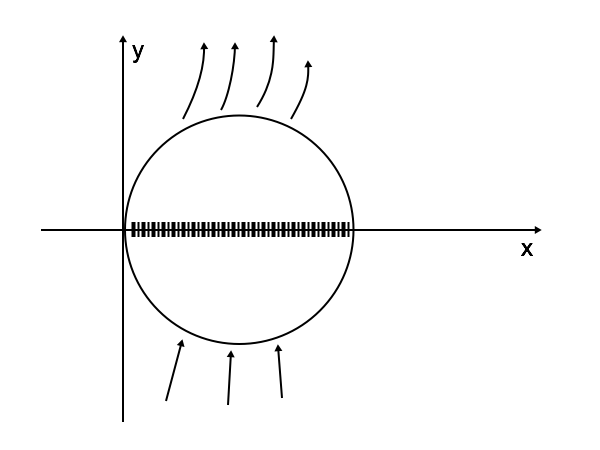
\includegraphics[width=0.6\textwidth]{lec13_circle_case1.png}
		 \end{center}
		 
		 Далее, двигаясь \underline{по оси $ Ox $} получаем, что 
		 $a = 0 \leq x \leq 2 = b$.
		 Потом начинаем двигаться в плоскости 
		 \underline{вдоль оси $ Oy $} и смотреть,
		 через какую границу мы входим в область и выходим из нее.
		 
		 В данном случае, рассматривая
		 $ T $ как криволинейную трапецию, вдоль оси $ Oy $ имеем:
		 \[ \left( x - 1\right)^2 + y^2 = 1 \implies 
		 y^2 = 1 - \left( x - 1 \right)^2 = 
		 2x - x - x^2 \implies y = \pm \sqrt{ 2x - x^2 } \]
		 
		 Вход: $ -\sqrt{2x - x^2 }$.
		 
		 Выход: $ y = \sqrt{2x - x^2 } $.
		 
		 Получаем
		 
		 \[ I = \int\limits_0^2 dx \int\limits_{-\sqrt{2x - x^2}} ^ 
		 {\sqrt{2x - x^2}} f \left( x, y\right) dy. \]
		\item Будем рассматривать $ T $ как криволинейную трапецию вдоль оси $ Ox $.
		В этом случае, действуя аналогично, проецируя область на ось $ Oy $, имеем 
		$ -1 \leq y \leq 1$. Двигаясь вдоль оси $ Ox $ слева направо 
		имеем границу входа в левую полуокружность:
		
		\[ \left( x - 1 \right)^2 + y^2 = 1 \implies x = 1 \pm \sqrt{1 - y^2} \]
		
		Вход: $ x = 1 - \sqrt{1 - y^2 }$.
		
		Выход: $ x = 1 + \sqrt{1 - y^2 } $.
		
		\begin{center}
			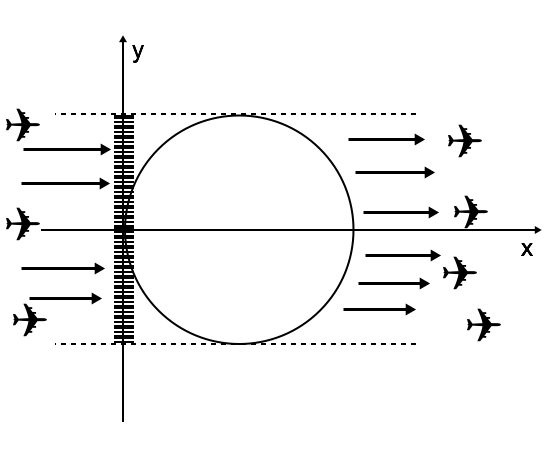
\includegraphics[width=0.6\textwidth]{lec13_circle_case2.png}
		\end{center}
		
		\[ I = \int\limits_{-1}^1 dy \int\limits_{1 - \sqrt{1 - y^2}} ^ 
		{1 + \sqrt{1 - y^2}} f \left( x, y\right) dx. \]
	\end{enumerate}
\end{exmp}

На практике для представления 2И через повторные интегралы
в случае
сложных областей интегрирования, разбивают области горизонтальными
прямыми на соответствующие криволинейные трапеции вдоль осей $Ox$ и $Oy$.
Если это удается
и число трапеций конечное, то используют аддитивность 2И и рассматривают
каждую из этих частей в отдельности.

\section{Тройной интеграл (3И)}

Рассмотрим Ф3П $ f \left( x, y, z \right)$, определенную для 
$\forall x, y, z \in H $~--- измеримое множество в $ \R^3 $
(кубируемое тело). В данном случае имеем \emph{тройной интеграл} (3И):

\begin{equation}
\label{lec_13, num_23}
I = \iiint\limits_{H} f \left( x, y, z \right) dx dy dz.
\end{equation}

\end{document}
